
\documentclass[preprint,12pt]{elsarticle}

\usepackage[spanish]{babel}
\usepackage{amssymb}
\usepackage{graphicx}
\usepackage{lineno}
\usepackage[utf8]{inputenc}
\usepackage{url}
\usepackage{color}
\usepackage{enumerate} 
\usepackage[hidelinks]{hyperref}


\begin{document}
	
	\begin{frontmatter}
		
		
		\title{\huge Metodología Inmon vs Metodología Kimball}
		
		\author{Mamani Ayala, Brandon        (2015052715)}
		\author{Quispe Mamani, Angelo	      (2015052826)}
		\author{Vizcarra Llanque, Jhordy	      (2015052719)}
		\author{Ordoñez Quilli, Ronald          (2015052821)}
		\author{Rodriguez Mamani, Juan      (2017057862)}
		
		\address{Tacna, Perú}
		
		\begin{abstract}
			%% Text of abstract
			
The data warehouses in English take each importance day, as organizations move from schemes of only data collection to schemes of analysis of the same. However, in spite of the great diffusion of the concepts related to data warehouses, there is not too much Information available in Spanish regarding the methodologies fo implement them In this short article we will try to provide a general explanation of one of the most used methodologies, the Kimball methodology 
		\end{abstract}
\end{frontmatter}
%%

	
	%%
	%\linenumbers
	
	%% main text
	\section{Resumen}
Los almacenes de datos (data warehouses en inglés) toman cada día mayor importancia, a medida que las organizaciones pasan de esquemas de sólo recolección de datos a esquemas de análisis de los mismos. Sin embargo a pesar de la gran difusión de los conceptos relacionados con los almacenes de datos, no existe demasiada información disponible en castellano en cuanto a las metodologías para implementarlos. En este breve artículo intentaremos brindar una explicación general de una de las metodologías más usadas, la metodología de Kimball \\
	%%
	
	%%
	%\linenumbers
	
	%% main text

\section{Objetivos}

	%%
	
	%%
	%\linenumbers
	
	%% main text

\section{Marco Teorico}

\begin{enumerate}[3.1]
    \item Introduccion. \\
\\
Un almacen de datos (data warehouse, DW) segun Inmon (Inmon 02, Imhoff y Galemmo 03), es una colecci\'on de datos orientada a un determinado \'ambito (empresa, organización, etc.), integrado, no volátil y variable en el tiempo, que ayuda a la toma de decisiones en la entidad en la que se utiliza. Se trata, sobre todo, de un historial completo de la organización, más allá de la información transaccional y operacional, almacenado en una base de datos diseñada para favorecer el análisis y la divulgación eficiente de datos (especialmente con herramientas OLAP, de procesamiento analítico en línea). Por otra parte Kimball (Kimball 98) la define como “una copia de los datos transaccionales estructurados específicamente para consultas y analisis”. Actualmente uno de los mayores impedimentos para construir este tipo de almacenes de datos es la falta de conocimiento de metodologías adecuadas para su implementación, y la disciplina para cumplirlas. En este breve art\'iculo describiremos la metodología más utilizada actualmente: la metodología de Kimball.

    \item Metodologias Actuales \\
\\
 Existen muchas metodologías de diseño y construcción de DW. Cada fabricante de software de inteligencia de negocios busca imponer una metodología con sus productos. Sin embargo, se imponen entre la mayoría dos metodologías, la de Kimball y la de Inmon. Para comprender la mayor diferencia entre estas dos metodologías, debemos explicar además de la noción de DW mencionando en la introducción, la idea de Data mart. Un Data mart (Kimball et al 98) es un repositorio de información, similar a un DW, pero orientado a un área o departamento específico de la  organización (por ejemplo Compras, Ventas, RRHH, etc.), a diferencia del DW que cubre toda la organización, es decir la diferencia fundamental es su alcance.
Desde el punto de vista arquitectónico, la mayor diferencia entre los dos autores es el sentido de la construcción del DW, esto es comenzando por los Data marts o ascendente (Bottom-up, Kimball) o comenzando con todo el DW desde el principio, o descendente.
Por otra parte, la metodología de Inmon se basa en conceptos bien conocidos del diseño de bases de datos relacionales (Inmon 02, Imhoff y Galemmo 03) la metodología para la construcción de un sistema de este tipo es la habitual para construir un sistema de información, utilizando las herramientas habituales, al contrario de la de Kimball, que se basa en un modelado dimensional (no normalizado)

    \item Metodologia Kimball en detalle.\\
\\

La metodología se basa en lo que Kimball denomina Ciclo de Vida Dimensional del Negocio (Business Dimensional Lifecycle) (Kimball et al 98, 08, Mundy y Thornthwaite 06). Este ciclo de vida del proyecto de DW, está basado en cuatro principios básicos :
\begin{itemize}
  \item Centrarse en el negocio:  Hay que concentrarse en la identificación de los requerimientos del negocio y su valor asociado, y usar estos esfuerzos para desarrollar relaciones sólidas con el negocio, agudizando el análisis del mismo y la competencia consultiva de los implementadores.
\\
  \item Construir una infraestructura de informaci\'on adecuada: Diseña una base de información única, integrada, fácil de usar, de alto rendimiento donde se reflejará la amplia gama de requerimientos de negocio identificados en la empresa.\\
  \item Realizar entregas en incrementos significativos crear el almacén de datos (DW) en incrementos entregables en plazos de 6 a 12 meses. Hay que usa el valor de negocio de cada element identificado para determinar el orden de aplicación de los incrementos. En esto la metodología se parece a las metodologías ágiles de construcción de software.\\
  \item 
Ofrecer la solución completa proporcionar todos los elementos necesarios para entregar valor a los usuarios de negocios. Para comenzar, esto significa tener un almacén de datos sólido, bien diseñado, con calidad probada, y accesible. También se deberá entregar herramientas de consulta ad hoc, aplicaciones para informes y análisis. \\
\end{itemize} 

La construcción de una solución de DW/BI (Datawarehouse/Business Intelligence) es sumamente compleja, y Kimball nos propone una metodología que nos ayuda a simplificar esa complejidad. Las tareas de esta metodología (ciclo de vida) se muestran en la figura 1. 
De la figura 1, podemos observar dos cuestiones. Primero, hay que resaltar el rol central de la tarea de definición de requerimientos. Los requerimientos del negocio son el soporte inicial de las tareas subsiguientes. También tiene influencia en el plan de proyecto (nótese la doble fecha entre la caja de definición de requerimientos y la de planificación). En segundo lugar podemos ver tres rutas o caminos que se enfocan en tres diferentes áreas

\begin {center}
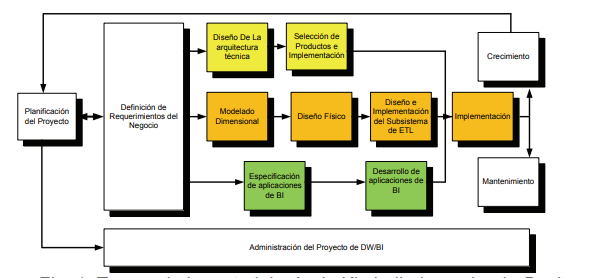
\includegraphics[scale= 0.80]{./Imagenes/1.png}
\end {center}

De la figura 1, podemos observar dos cuestiones. Primero, hay que resaltar el rol central de la tarea de definición de requerimientos.
Los requerimientos del negocio son el soporte inicial de las tareas subsiguientes. También tiene influencia en el plan de proyecto (nótese la doble fecha entre la caja de definición de requerimientos y la de planificación). En segundo lugar podemos ver tres rutas o caminos que se enfocan en tres diferentes áreas:\\

\begin{itemize}
  \item Tecnología (Camino Superior). Implica tareas relacionadas con software específico, por ejemplo, Microsoft SQL Analysis Services.
\\
  \item Datos (Camino del medio). En la misma diseñaremos e implementaremos el modelo dimensional, y desarrollaremos el subsistema de Extracción, Transformación y Carga (Extract, Transformation, and Load  ETL) para cargar el DW.
\\
  \item Aplicaciones de Inteligencia de Negocios (Camino Inferior). En esta ruta se encuentran tareas en las que diseñamos y desarrollamos las aplicaciones de negocios para los usuarios finales.
\\

\end{itemize} 
Estas rutas se combinan cuando se instala finalmente el sistema. En la parte de debajo de la figura se muestra la actividad general de administración del proyecto. A continuación describiremos cada una de las tareas. 
\end{enumerate}

\section{Ejemplo}

\section{Analisis}

\section{Conclusion}

%%
	
	%%
	%\linenumbers
	
	%% main text

	
	
	\newpage
	
		%ESTILO
	   \bibliography{BIBLIOGRAFIA}		%ARCHIVO .bib
	   \begin{thebibliography}{0}
                \bibitem{Ronald} https://twooctobers.com/blog/8-data-storytelling-concepts-with-examples/
                 \bibitem{Juan} https://twooctobers.com/blog/8-data-storytelling-concepts-with-examples
                  \bibitem{Jhordy} https://www.pqs.pe/campus-romero/data-storytelling-empresas
                  \bibitem{Jhordy} https://observatoriocibermedios.upf.edu/patterns-in-data-storytelling
                    \bibitem{Brandon} https://twooctobers.com/blog/8-data-storytelling-concepts-with-examples/
                   \bibitem{Brandon}https://www.ucasal.edu.ar/htm/ingenieria/cuadernos/archivos/5-p56-rivadera-formateado.pdf

         \end{thebibliography}

	
\end{document}

%%
%% End of file `elsarticle-template-1-num.tex'.
